\chapter{Handover Parameter Optimisation}\label{handover parameter optimisation}
\section{Approach}\label{approach}
The approach taken for optimising the handover parameters in LTE uses a Q-Learning algorithm based on the process given in Section~\ref{sec:qlearning}. In the approach the model of the environment has a state for every combination of TTT and hys; giving a total number of 336 states. An action within the model can move to any other state that is different by one of the following changes to the handover parameters:

\begin{enumerate}
	\item A single increase of TTT.
	\item A single increase of hys.
	\item A single increase of both TTT and hys.
	\item A single decrease of TTT.
	\item A single decrease of hys.
	\item A single decrease of both TTT and hys.
	\item A single value increase of TTT and a single value decrease of hys.
	\item A single value increase of hys and a single value decrease of TTT.
\end{enumerate}

For example if the learning agent is in the state where the TTT equals $0.256 s$ and the hys equals $5.0 dB$ and did action 3 from the list seen above; then the new TTT would equal $0.32 s$ and the hys would equal $5.5 dB$. The full list of hys values can be seen in Table~\ref{tab:hys} and the full list of TTT values can be seen in Table~\ref{tab:ttt}.

Having the actions only change the parameters by one increase or decrease of the TTT and hys values each time not only allows for more refined optimisation of the parameters but it also makes sure that no large changes can suddenly happen.

Due to the nature to the kind of problem that is being solved, the reward gained by an action is dynamic and is likely to be different each time it is taken. Rewards are based on the number of drop and ping-pong's accumulated in the simulation for current state in the environment model. The rewards are defined by the following equation:
\begin{equation}\label{eq:reward}
Reward = Handover_{successful} – (10*Drops + 2*PingPong's)
\end{equation}
The coefficients in Equation~\ref{eq:reward} are given the values of $10$ for drops and $2$ for ping-pong's. Drops are extremely bad for the QoS of a communication system so it's given a large value and the reason ping-pong's are multiplied by $2$ to remove the successful handover that was caused by the ping-pong and give the agent a penalty. The reward is given to the agent and the Q-Value for that state is updated just before agent selects the next action to take.  The agent then selects new actions in discrete time steps, this allows for the simulation to run for fixed periods of time with TTT-hys pairs specified by a state in the environment model. 

After the agent has been given enough time to try every action at least once the Q-Learning agent generates a policy. This policy can then be used to attempt to optimise the handover parameters by changing the TTT and hys values after a call is dropped or the connection ping-pongs between base stations. The Q-Learning agent still receives rewards every time a call is dropped or the connection ping-pong's while following the generated policy. Doing this allows for the system to always be learning; even after the initial learning process that generated the policy.

The optimisation system was tested in two scenarios. One scenario was to have 10 UE's moving randomly around 9 base stations, with the layout as seen in Figure (Place Holder), using the Random Direction mobility model seen in Section~\ref{mobility}, where the speed of the UE is $1$ to $4 m/s$, which is walking speed and the duration of the direction is between $100$ and $200$ seconds. The other scenario is to have the UE moving at $10$ to $15 m/s$, which is roughly $30 mph$.

Place holder for base station layout.

Each base station has its own Q-Learning agent to optimise the TTT and hys values for that specific base station. The agents are given 1000000 seconds to attempt to learn the environment that are working within, with each state being given 180 seconds to gain their reward. This length of time was chosen because there are 336 state each with a maximum of 8 actions, therefore the time needed to do all actions would take approximately 483840 seconds if each action was given 180 seconds. This length of time is less than half of the total time given so even due to the randomness of selecting next actions when learning the environment there should be enough time to try all state and most of the actions available. After the agents have learned the environment they generate a policy for their base station to follow. The simulation is then run for 200000 seconds to test how well the policies perform. The results for the scenarios can be seen in Section~\ref{results}.
\section{Results}\label{results}
To results are assessed by how well they performed compared to not making any changes to the TTT and hys values. The comparison is made by observing how to ratio of dropped calls and ping-pong's to successful handovers changes over time. The ratio of dropped calls is given by the following equation:
\begin{equation}\label{eq:drop}
Drop Ratio = \frac{\#Dropped Calls}{\#Successful Handovers}
\end{equation}
The ratio for the connection ping-ponging between base stations is given by the following equation:
\begin{equation}\label{eq:ping}
PingPong Ratio = \frac{\#PingPong's}{\#Successful Handovers}
\end{equation}
It is also important to see how the TTT and hys values are being changes when the system is attempting to optimise them. This will allows it to be seen if the agents for the base stations come to some kind of consensus on the most optimal values of TTT and hys or if them come up with there own unique solutions. It is likely that Base Station 4 whose coverage overlaps with the coverage from every other Base Station, as seen in Figure (place holder), will come up with a different solution to the other Base Stations because it will be involved in the most handover attempts.

The simulation is run for four different starting states when compiling results for the UE moving at walking or vehicle speeds. The first starting state was to have the TTT and hys both start at their maximum values, 5.12 second and 10 dB respectively, to see how the system attempted to optimise the values as it is expected that a lot of dropped calls would occur for this set of values. The second start state was to give the TTT and hys their middle values, which are 0.256 seconds for TTT and 5 dB for hys. This start state would be expected to perform relatively well without any optimisation taking place due to the values neither being very large or very small. The third start state has the TTT and hys being at their lowest possible values of 0 seconds for TTT and 0 dB for hys. This starting state is expected to cause ping-pong's to occur because a handover will be triggered as soon as a neighbouring Base Station becomes better than the serving Base Station, instead of waiting to see if the neighbouring Base Station continues to be better for a period of time. The final starting start is to have the TTT start at a low value of 0.08 seconds and the hys start at a high value of 7.5 dB. This type of state was chosen to see how the well the system can optimise the values when it is likely that one will need to be increased and the other decreased.
\subsection{Walking Speed}
\subsubsection*{Large Values}
The results of how the optimised values compared to the static values can be seen in Figure~\ref{fig:walk_high_drop} when both the TTT and hys started with their largest possible values of 5.12 seconds and 10 dB respectively. The results show that while the process of optimising the values initially generated a very large increase in the number of dropped calls. However, the system then managed to improve rapidly and ended up having a better dropped call ratio by the end to the simulation run than that of the non-optimised system.
\begin{figure}[H]
  \begin{center}
    	  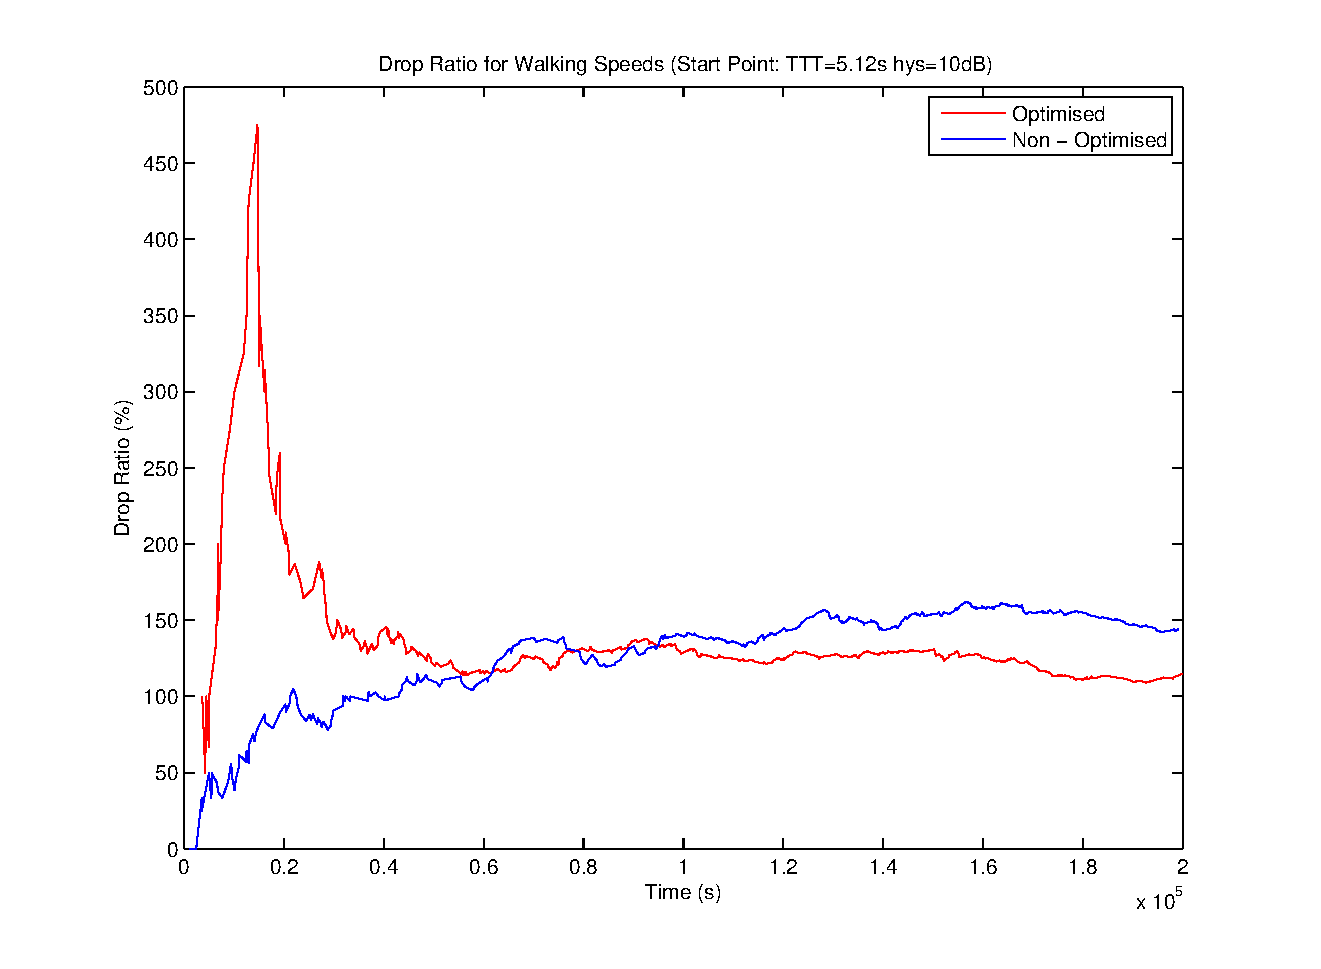
\includegraphics[width=0.75\textwidth]{figures/walking_figures/high/long_drop.eps}
    \end{center}
    \caption{Graph of Optimised vs. Non-Optimised Results for Starting Point TTT=5.12s hys=10dB when UE traveling at walking speeds.}
    \label{fig:walk_high_drop}
\end{figure}
Figure~\ref{fig:walk_high_ttt} shows how the TTT values were optimised over the course of the simulation run. It can be seen that all the base stations were in consensus that 5.12 seconds is too large of a values of the TTT and very quickly lowered the value. After this however there were effectively two different groups. The first group made up of base stations 1, 3, 4 and 5 ended up keeping the TTT value over 1 second. While the other group made up of base stations 0, 2, 6, 7 and 8 kept reducing the value to a most 0.48 seconds. It could be said that first group of base stations may not have optimised the TTT value as well as the second group because it can be seen that base stations 1, 4 and 5 kept switching between only two values when dropped calls occurred. It can also be seen the these changes happened often meaning that these base stations were still have dropped calls occurring, so it cannot be said that these values performed as well as those the base stations is the second group were using.
While the changes made to the TTT value could be split up into two different groups the same cannot be said for the changes made to the hys value as seen in Figure~\ref{fig:walk_high_hys}. It can be seen that while most of the base stations kept the hys value above 9 dB, base stations 0, 6, 7 and 8 lower the value more, with base station 8 settling between 5 and 5.5 dB. It can also be seen that base stations 1 and 3 appear to have gotten stuck between two non-optimal values as they keep switching between them and due to it happening often it means that dropped calls are still occurring so the system should have switched to different values to see if they had performed better.
\begin{figure}[H]
        \centering
        \begin{subfigure}[b]{0.49\textwidth}
                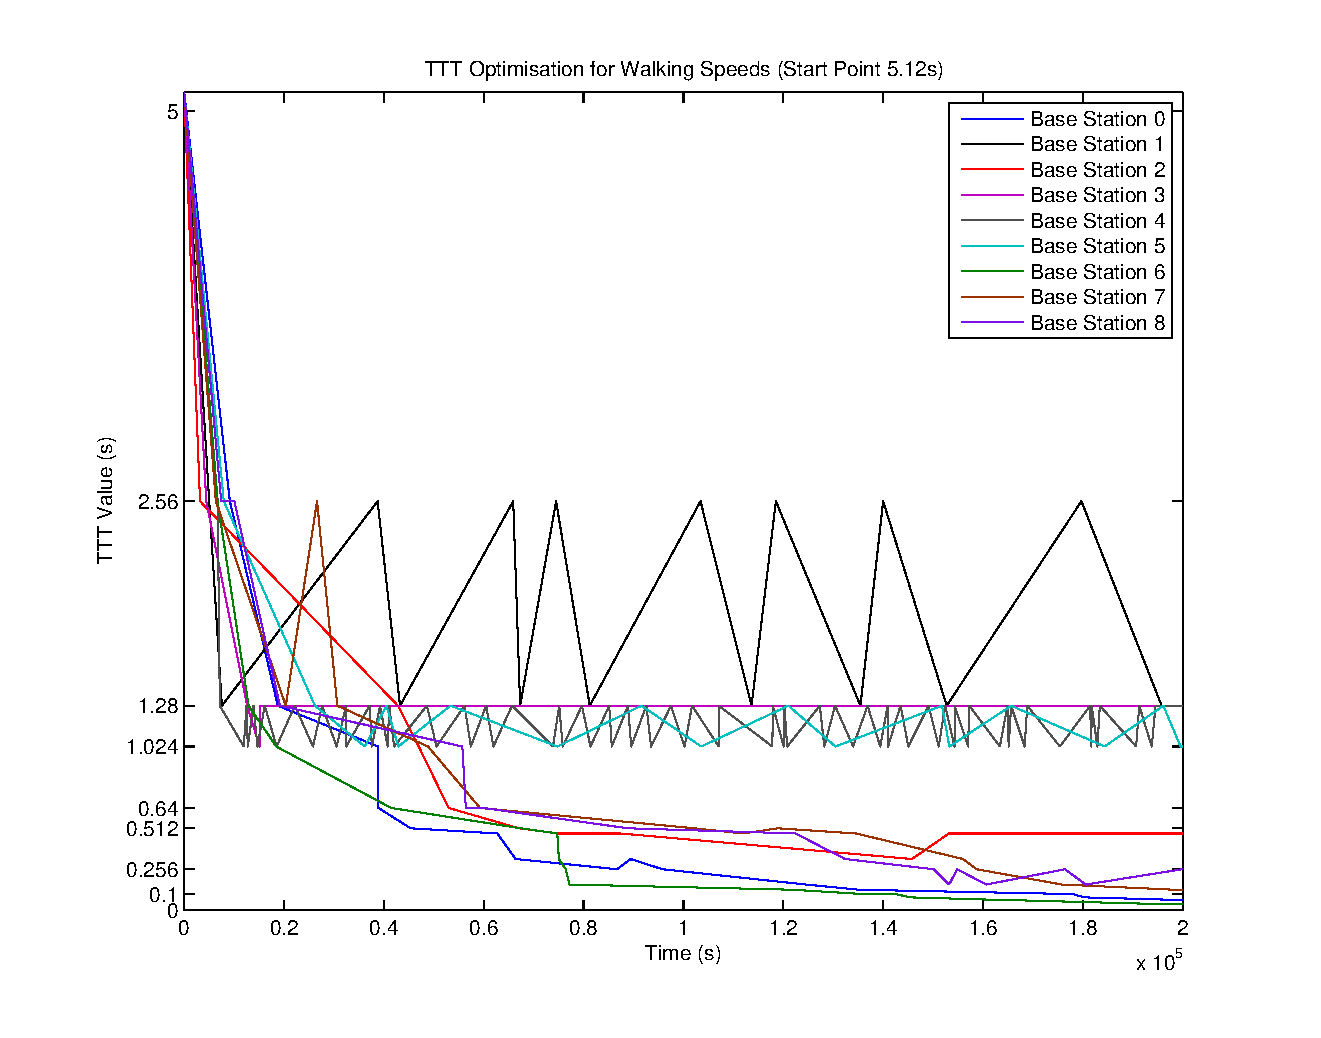
\includegraphics[width=\textwidth]{figures/walking_figures/high/long_ttt.eps}
                \caption{Changing TTT Values}
                \label{fig:walk_high_ttt}
        \end{subfigure}%
        ~ %add desired spacing between images, e. g. ~, \quad, \qquad etc.
          %(or a blank line to force the subfigure onto a new line)
        \begin{subfigure}[b]{0.49\textwidth}
                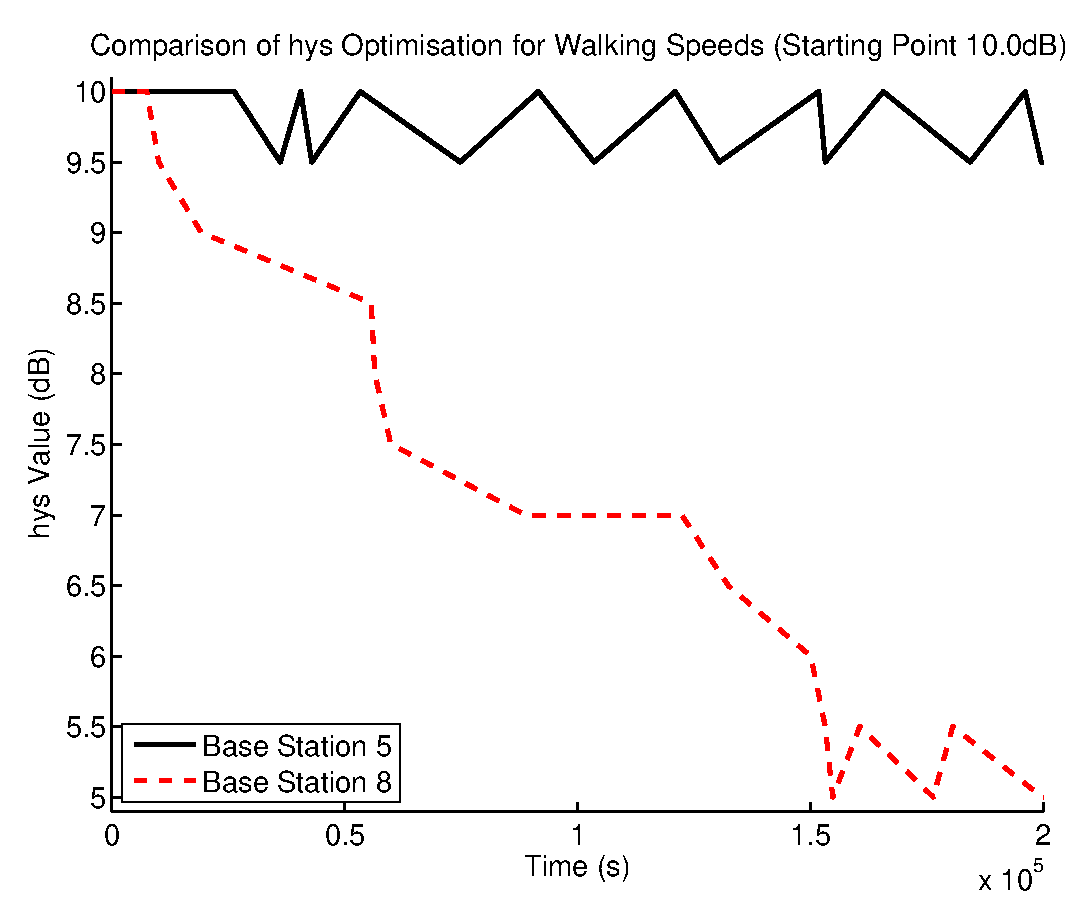
\includegraphics[width=\textwidth]{figures/walking_figures/high/long_hys.eps}
                \caption{Changing hys Values}
                \label{fig:walk_high_hys}
        \end{subfigure}
        \caption{Illustration of how the TTT and hys values changed over time for large values when UE traveling at walking speeds.}\label{fig:walk_high_ttthys}
\end{figure}

\subsubsection*{Medium Values}
\begin{figure}[H]
  \begin{center}
    	  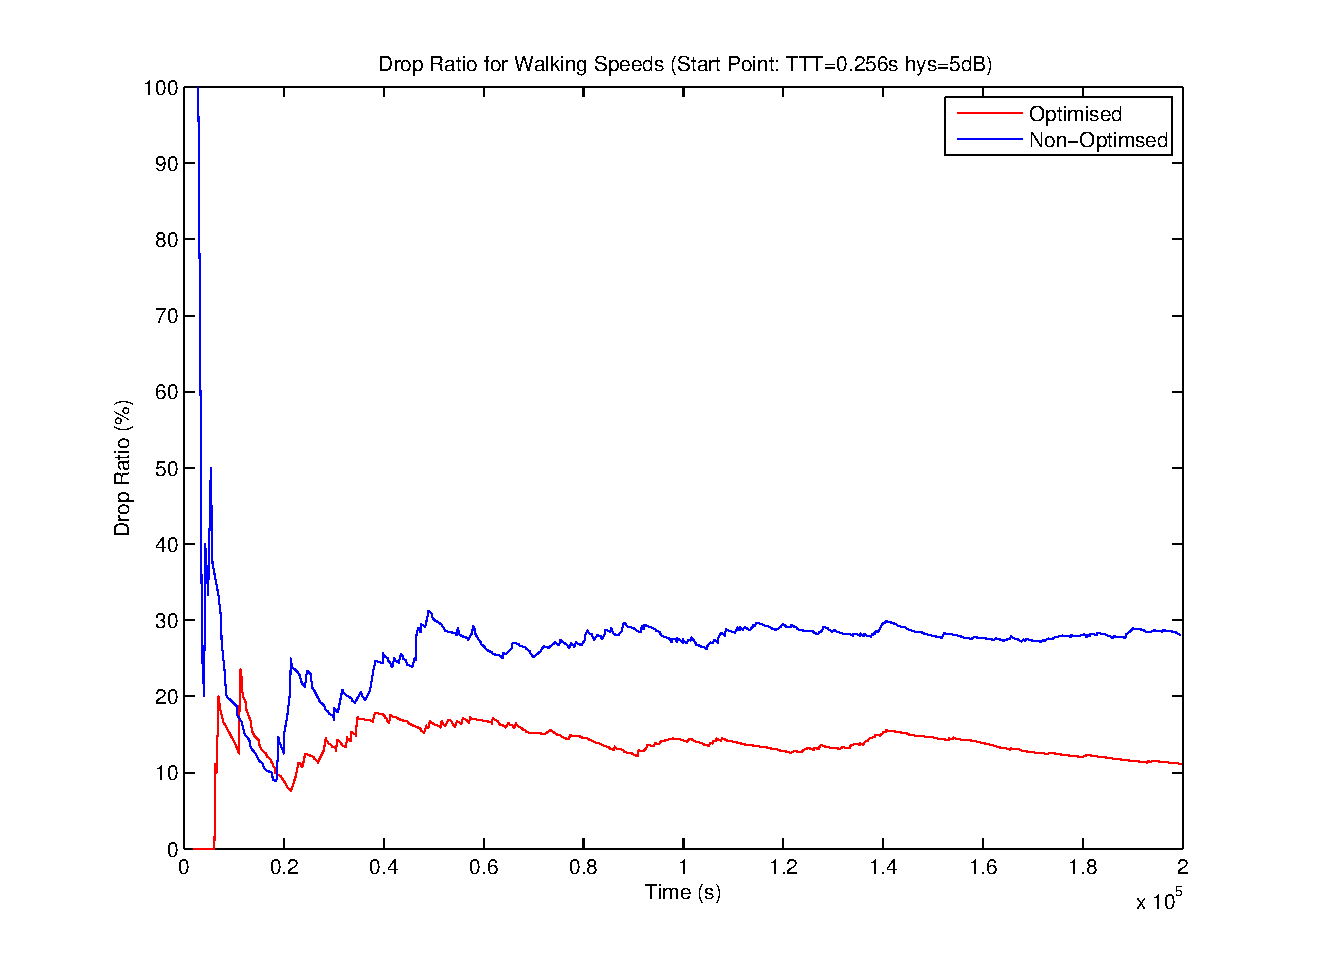
\includegraphics[width=0.75\textwidth]{figures/walking_figures/mid/long_drop.eps}
    \end{center}
    \caption{Graph of Optimised vs. Non-Optimised Results for Starting Point TTT=0.256s hys=5dB when UE traveling at walking speeds.}
    \label{fig:walk_mid_drop}
\end{figure}

\begin{figure}[H]
        \centering
        \begin{subfigure}[b]{0.49\textwidth}
                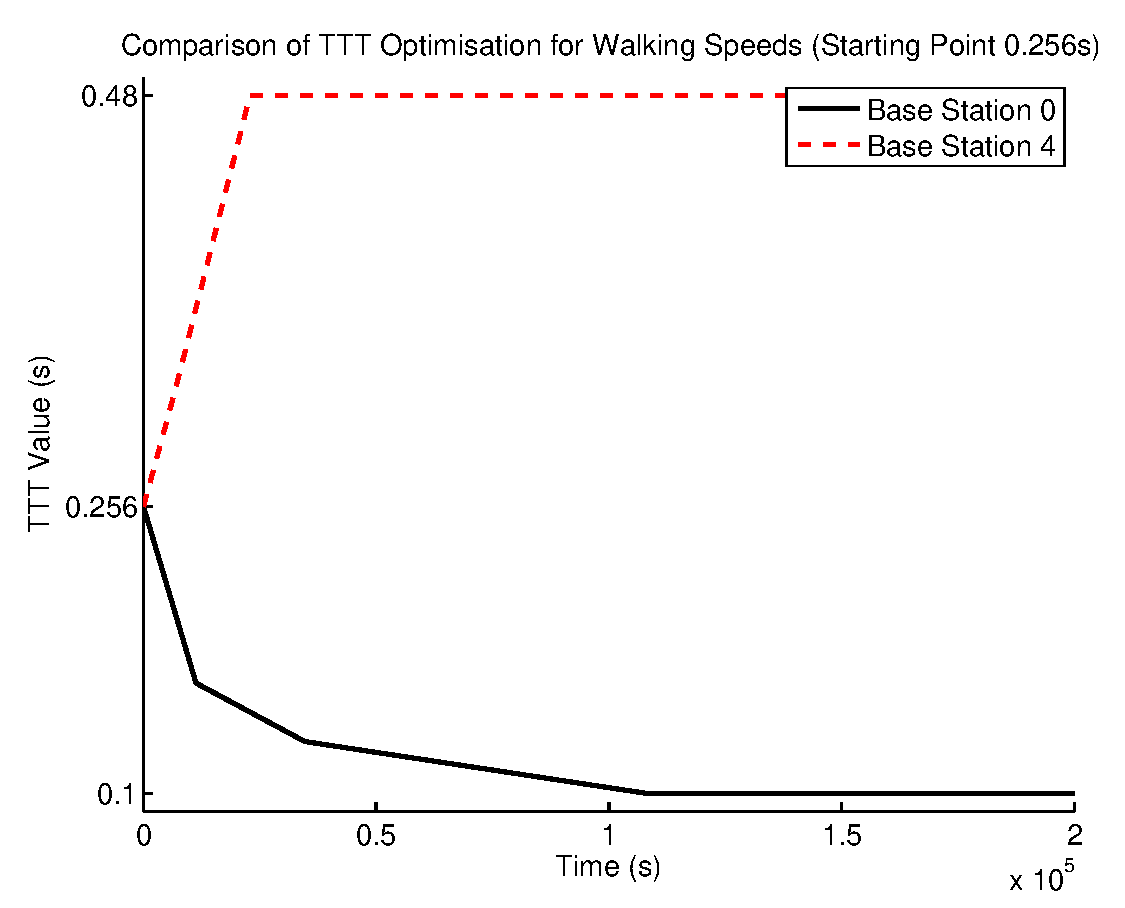
\includegraphics[width=\textwidth]{figures/walking_figures/mid/long_ttt.eps}
                \caption{Changing TTT Values}
                \label{fig:walk_mid_ttt}
        \end{subfigure}%
        ~ %add desired spacing between images, e. g. ~, \quad, \qquad etc.
          %(or a blank line to force the subfigure onto a new line)
        \begin{subfigure}[b]{0.49\textwidth}
                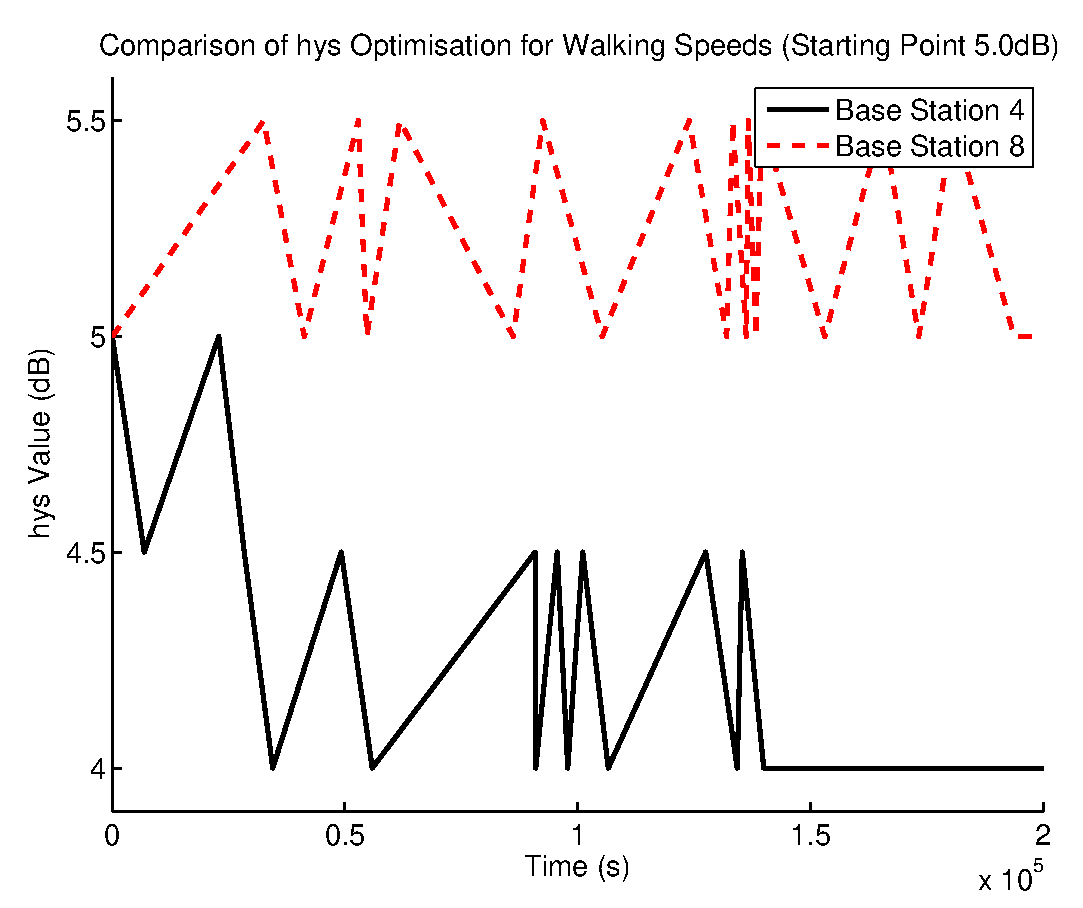
\includegraphics[width=\textwidth]{figures/walking_figures/mid/long_hys.eps}
                \caption{Changing hys Values}
                \label{fig:walk_mid_hys}
        \end{subfigure}
        \caption{Illustration of how the TTT and hys values changed over time for medium values when UE traveling at walking speeds.}\label{fig:walk_mid_ttthys}
\end{figure}

\subsubsection*{Small Values}
\begin{figure}[H]
  \begin{center}
    	  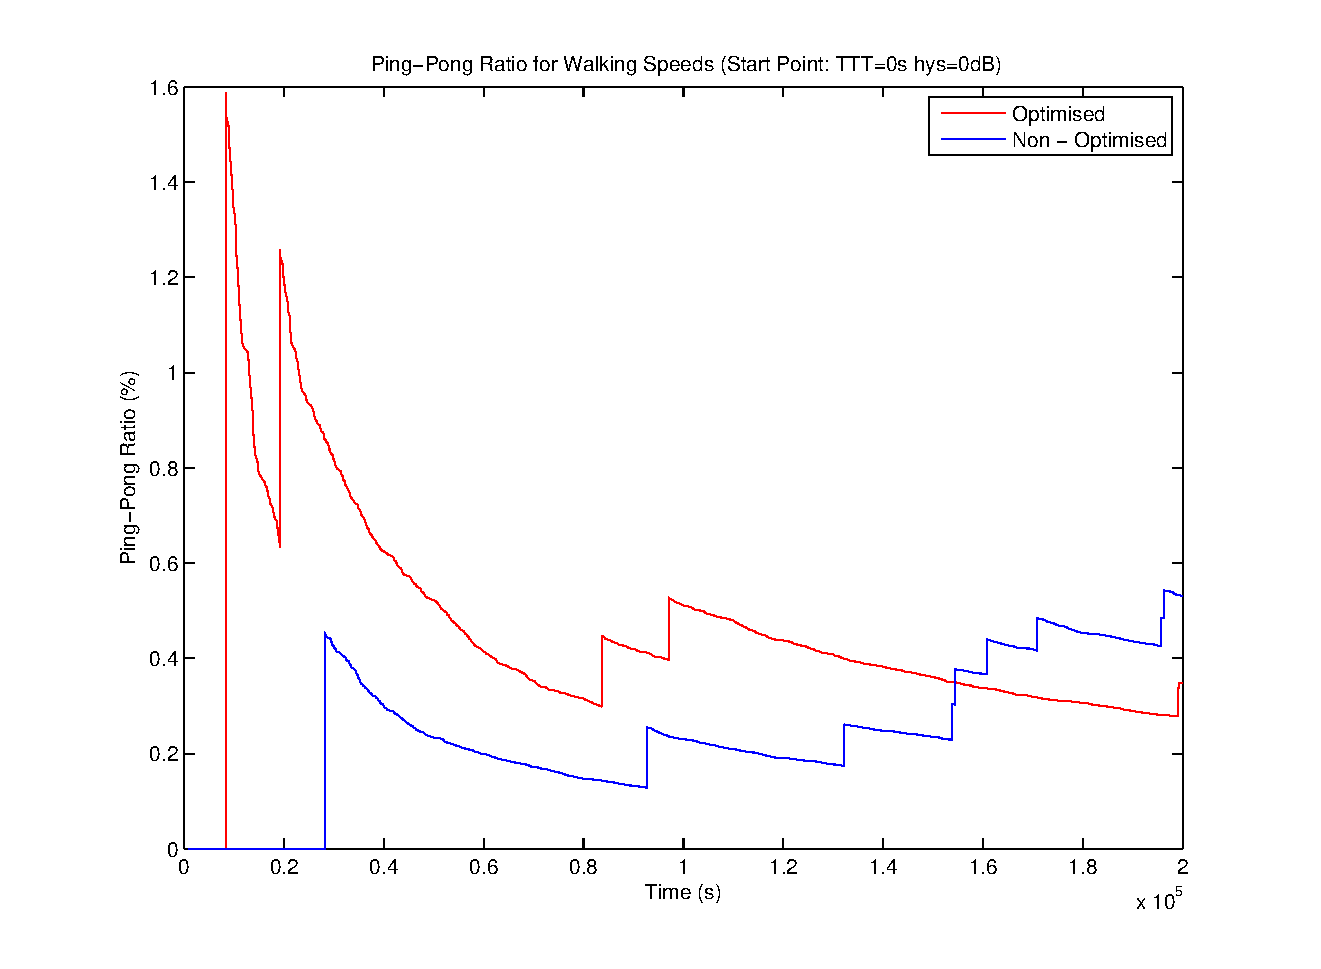
\includegraphics[width=0.75\textwidth]{figures/walking_figures/low/long_ping.eps}
    \end{center}
    \caption{Graph of Optimised vs. Non-Optimised Results for Starting Point TTT=0s hys=0dB when UE traveling at walking speeds.}
    \label{fig:walk_low_drop}
\end{figure}

\begin{figure}[H]
        \centering
        \begin{subfigure}[b]{0.49\textwidth}
                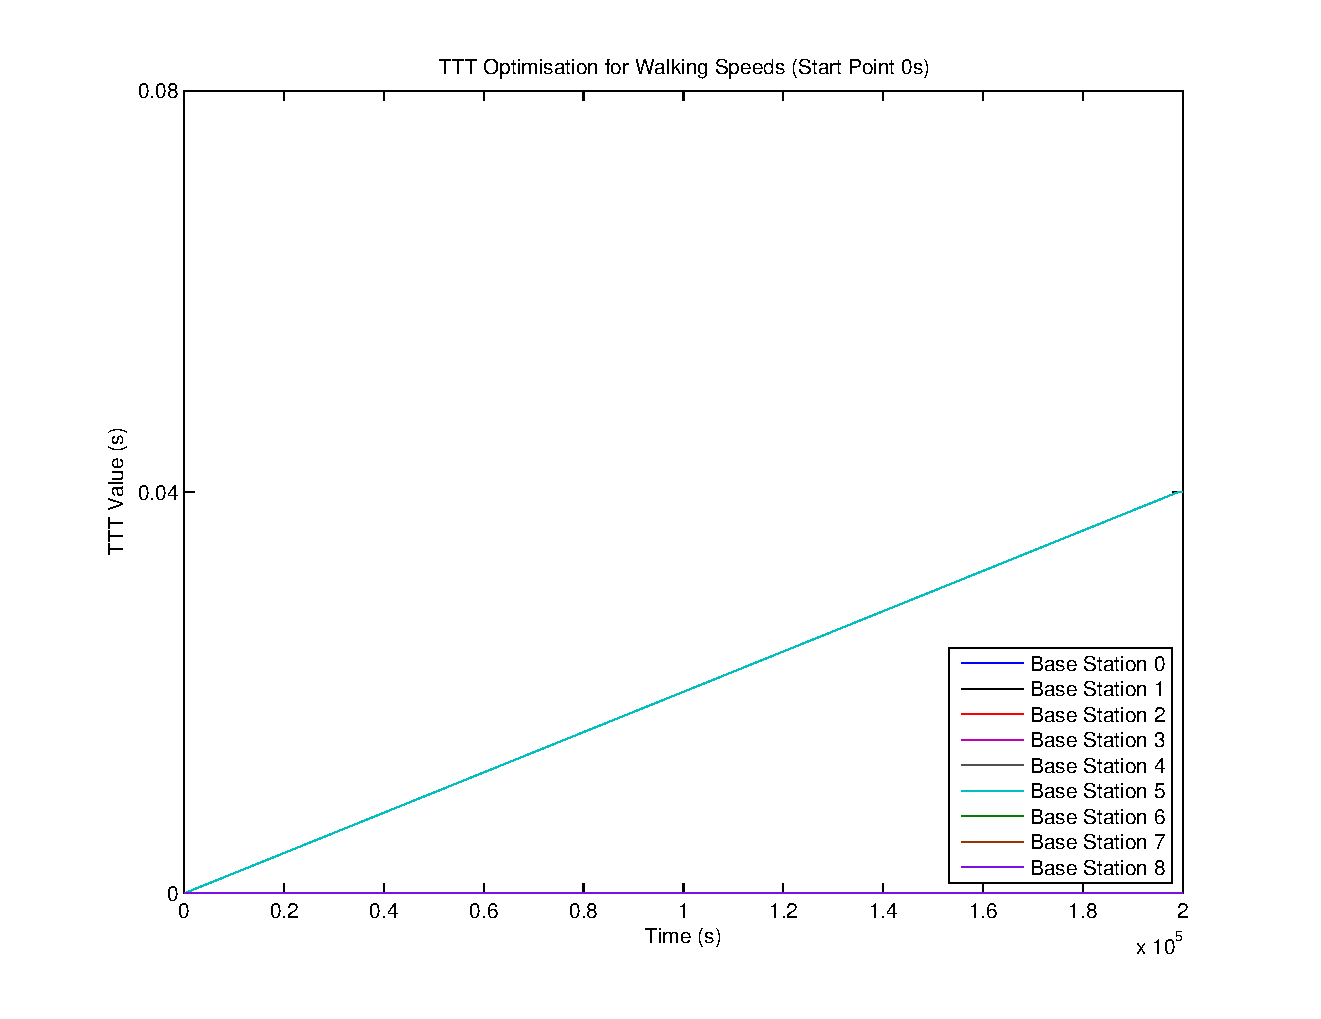
\includegraphics[width=\textwidth]{figures/walking_figures/low/long_ttt.eps}
                \caption{Changing TTT Values}
                \label{fig:walk_low_ttt}
        \end{subfigure}%
        ~ %add desired spacing between images, e. g. ~, \quad, \qquad etc.
          %(or a blank line to force the subfigure onto a new line)
        \begin{subfigure}[b]{0.49\textwidth}
                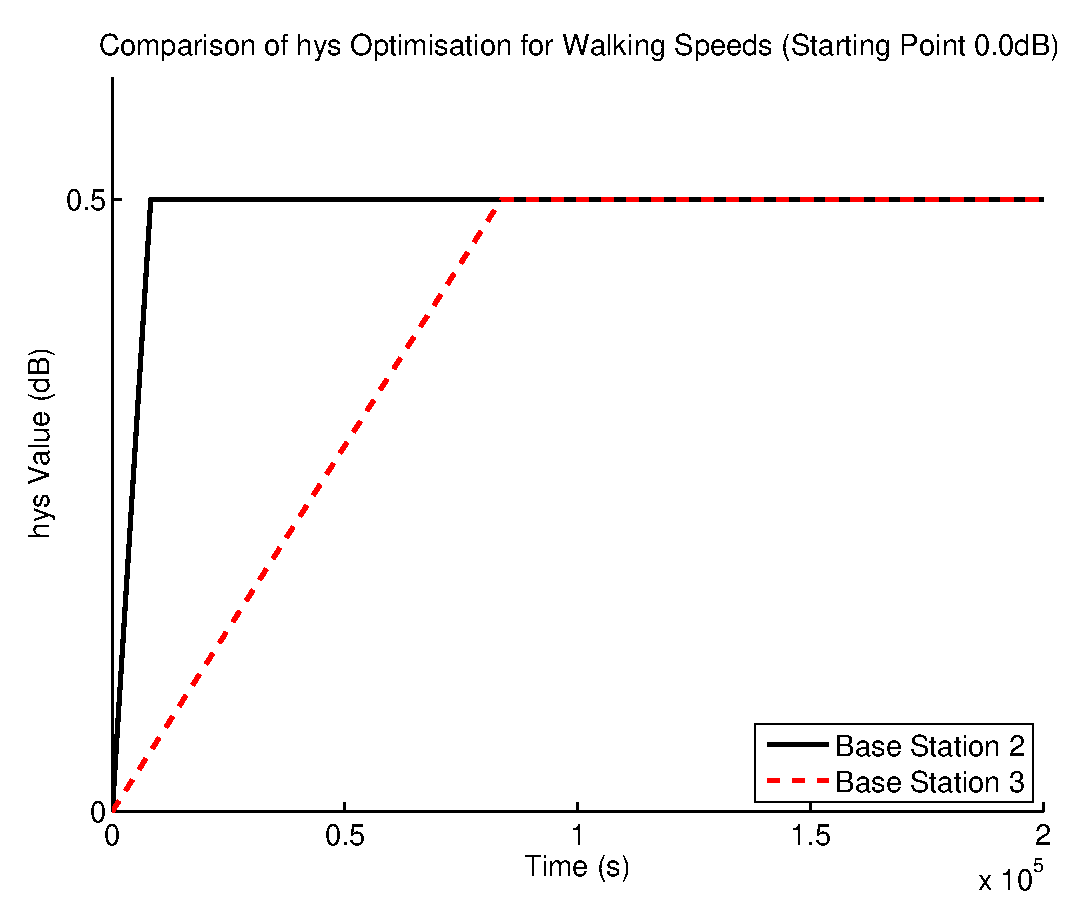
\includegraphics[width=\textwidth]{figures/walking_figures/low/long_hys.eps}
                \caption{Changing hys Values}
                \label{fig:walk_low_hys}
        \end{subfigure}
        \caption{Illustration of how the TTT and hys values changed over time for medium values when UE traveling at walking speeds.}\label{fig:walk_low_ttthys}
\end{figure}

\subsubsection*{Large hys and Small TTT Values}
\begin{figure}[H]
  \begin{center}
    	  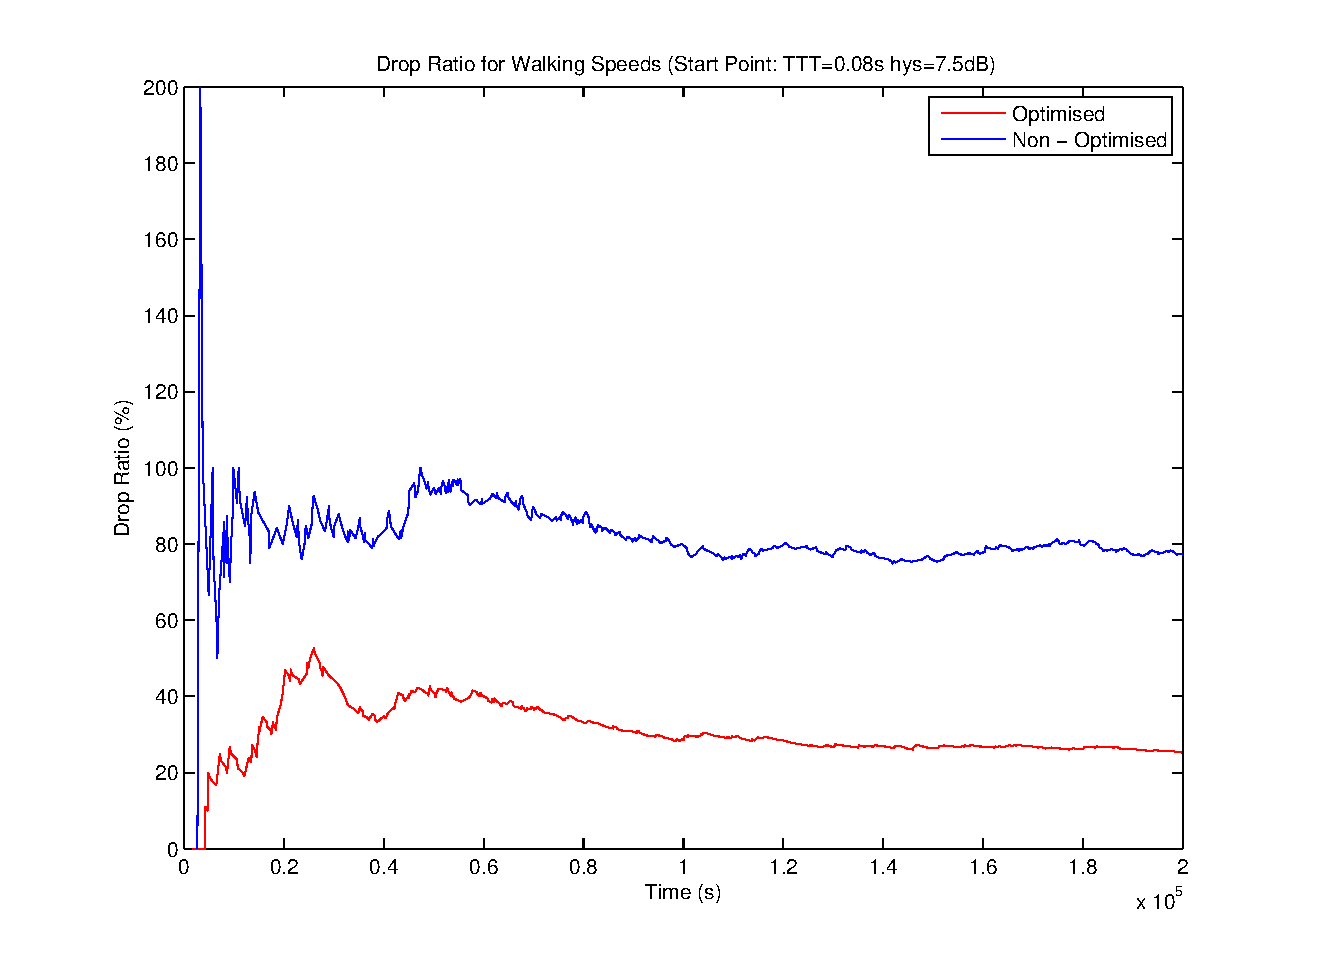
\includegraphics[width=0.75\textwidth]{figures/walking_figures/highhys/long_drop.eps}
    \end{center}
    \caption{Graph of Optimised vs. Non-Optimised Results for Starting Point TTT=0.08s hys=7.5dB when UE traveling at walking speeds.}
    \label{fig:walk_highhys_drop}
\end{figure}

\begin{figure}[H]
        \centering
        \begin{subfigure}[b]{0.49\textwidth}
                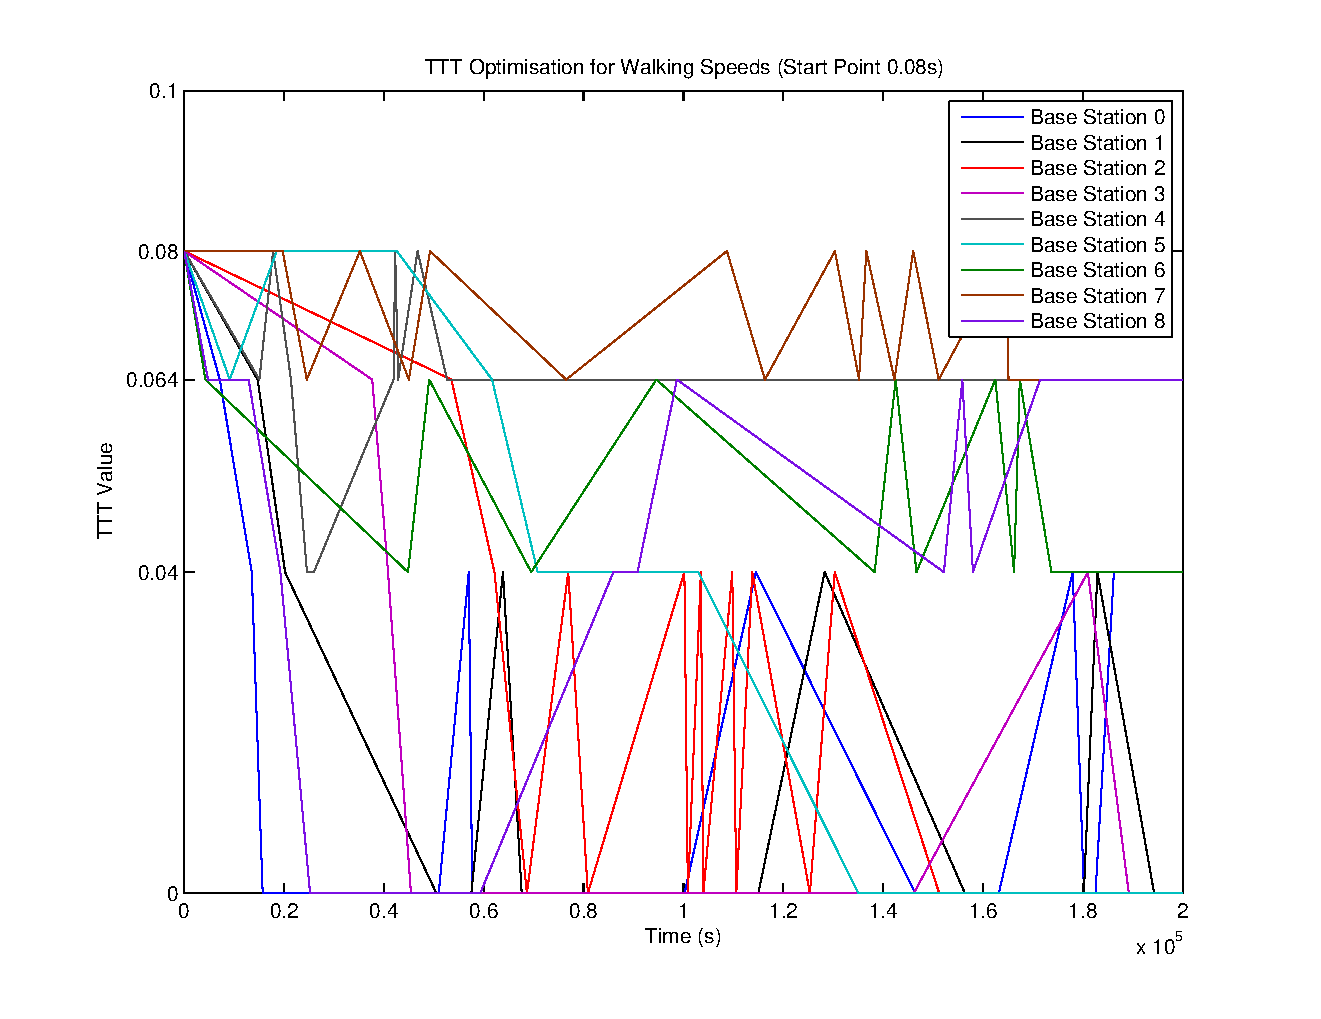
\includegraphics[width=\textwidth]{figures/walking_figures/highhys/long_ttt.eps}
                \caption{Changing TTT Values}
                \label{fig:walk_highhys_ttt}
        \end{subfigure}%
        ~ %add desired spacing between images, e. g. ~, \quad, \qquad etc.
          %(or a blank line to force the subfigure onto a new line)
        \begin{subfigure}[b]{0.49\textwidth}
                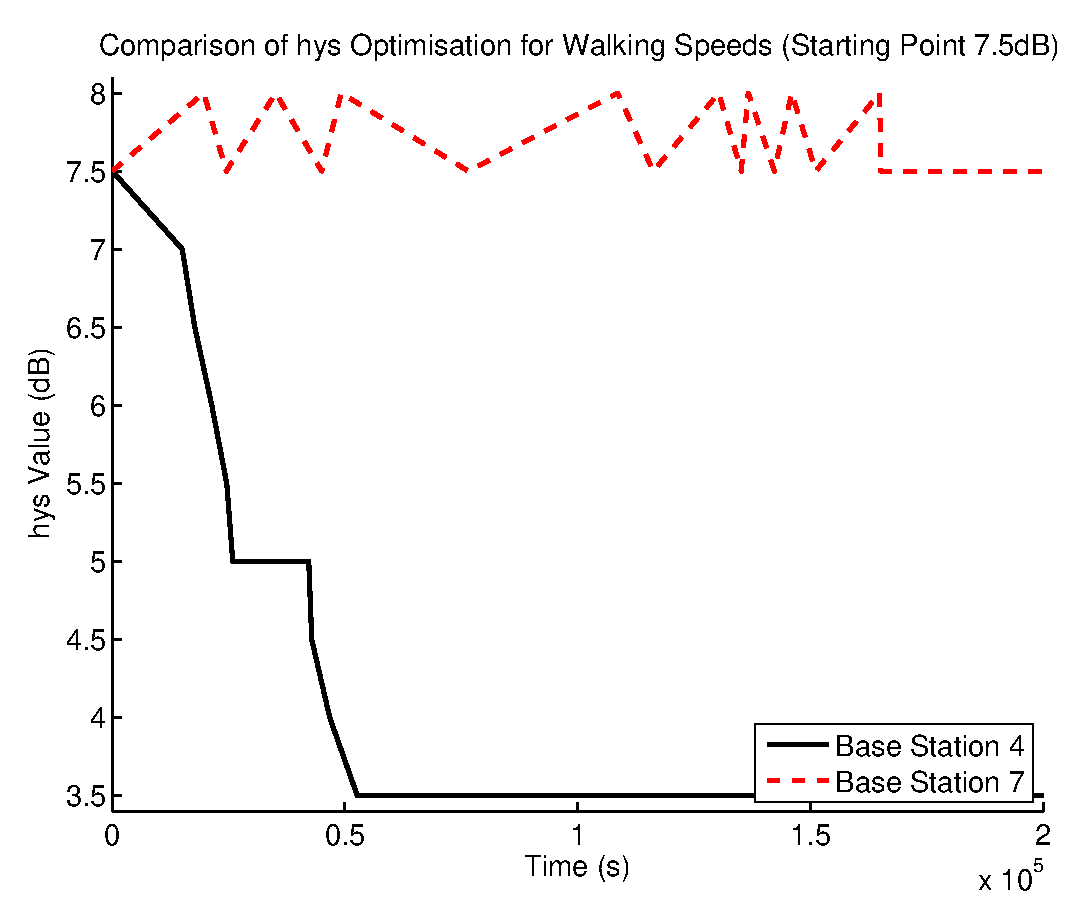
\includegraphics[width=\textwidth]{figures/walking_figures/highhys/long_hys.eps}
                \caption{Changing hys Values}
                \label{fig:walk_highhys_hys}
        \end{subfigure}
        \caption{Illustration of how the TTT and hys values changed over time for medium values when UE traveling at vehicle speeds.}\label{fig:walk_highhys_ttthys}
\end{figure}

\subsection{Vehicle Speed}
\subsubsection*{Large Values}
\begin{figure}[H]
  \begin{center}
    	  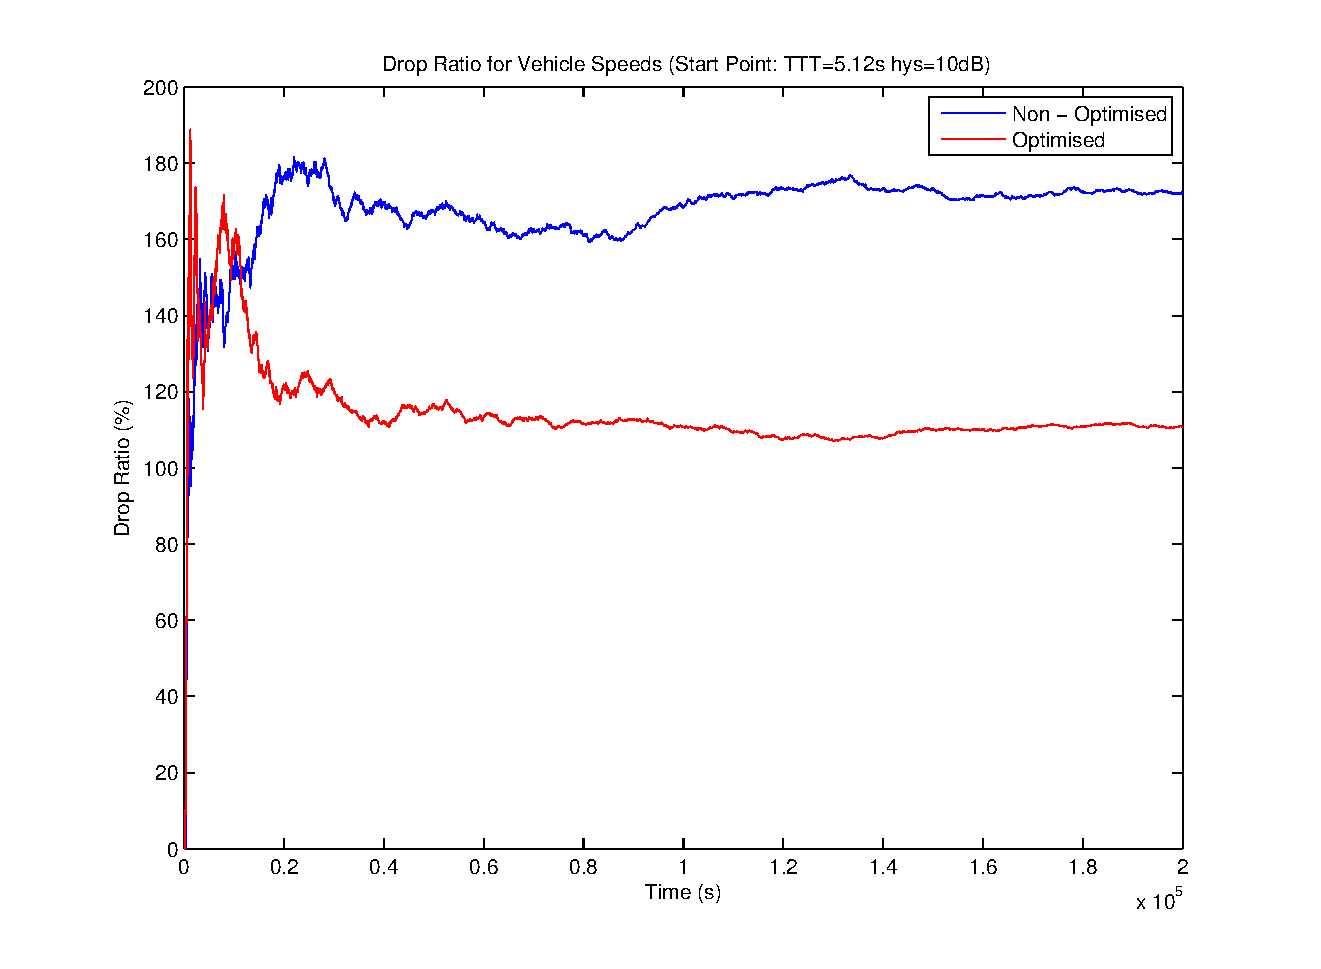
\includegraphics[width=0.75\textwidth]{figures/vehicle_figures/high/long_drop.eps}
    \end{center}
    \caption{Graph of Optimised vs. Non-Optimised Results for Starting Point TTT=5.12s hys=10dB when UE traveling at walking speeds.}
    \label{fig:veh_high_drop}
\end{figure}

\begin{figure}[H]
        \centering
        \begin{subfigure}[b]{0.49\textwidth}
                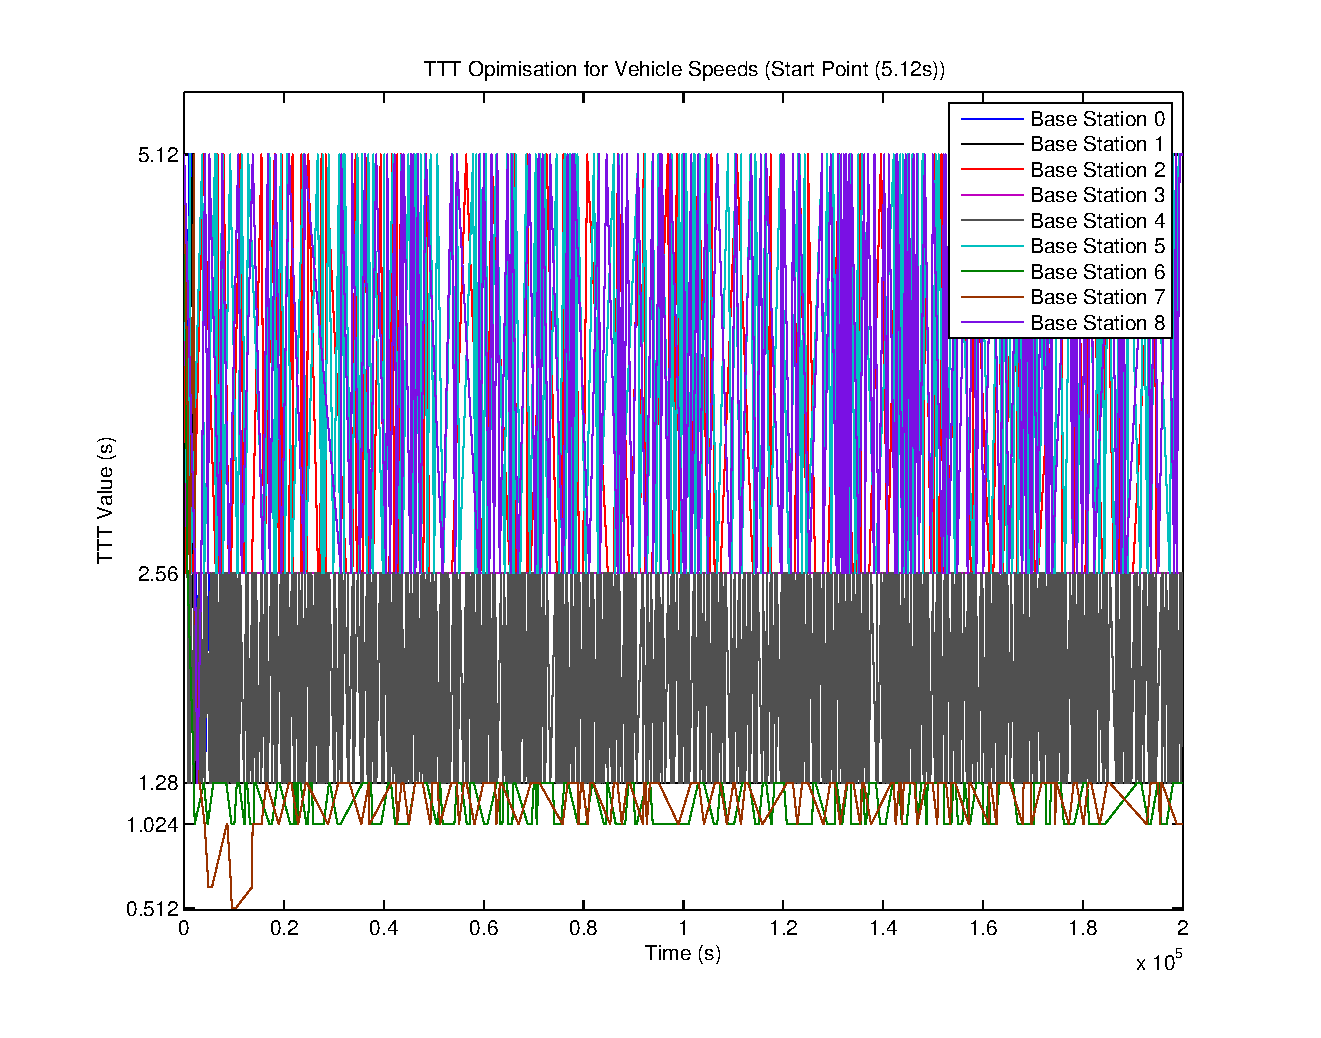
\includegraphics[width=\textwidth]{figures/vehicle_figures/high/long_ttt.eps}
                \caption{Changing TTT Values}
                \label{fig:veh_high_ttt}
        \end{subfigure}%
        ~ %add desired spacing between images, e. g. ~, \quad, \qquad etc.
          %(or a blank line to force the subfigure onto a new line)
        \begin{subfigure}[b]{0.49\textwidth}
                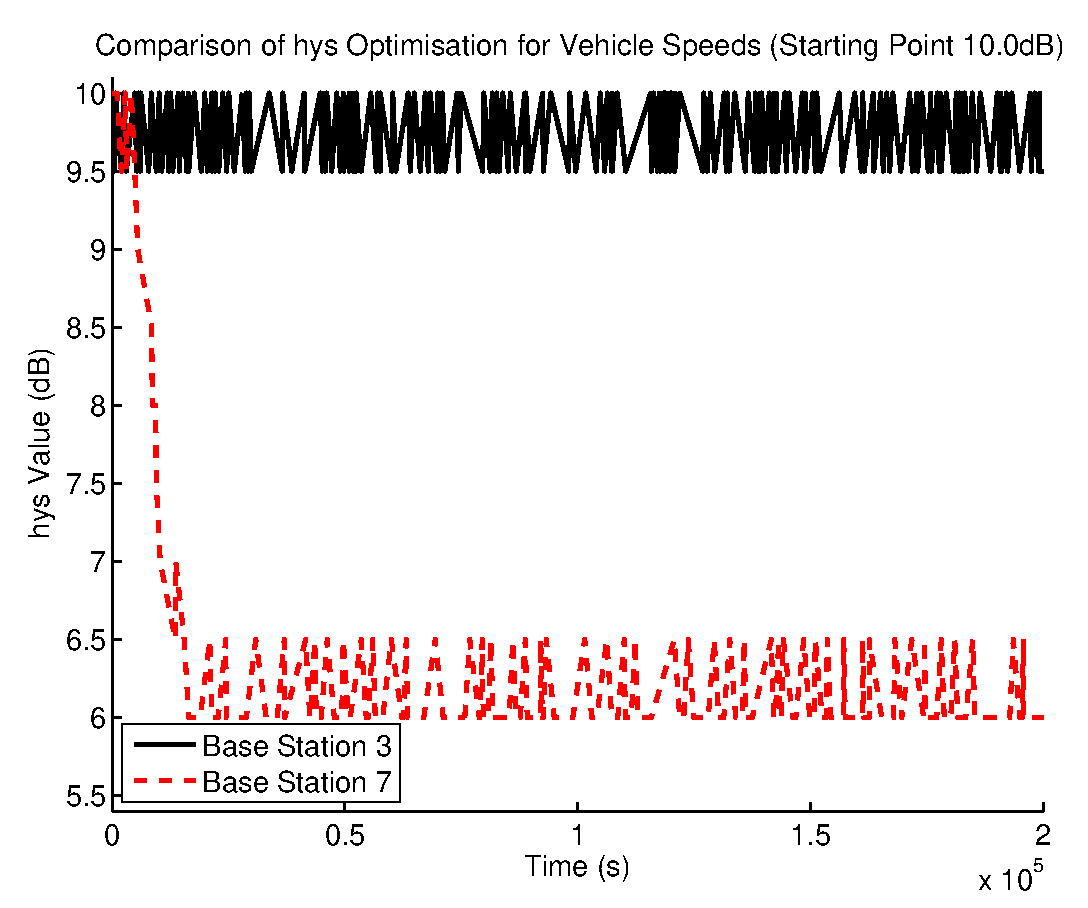
\includegraphics[width=\textwidth]{figures/vehicle_figures/high/long_hys.eps}
                \caption{Changing hys Values}
                \label{fig:veh_high_hys}
        \end{subfigure}
        \caption{Illustration of how the TTT and hys values changed over time for large values when UE traveling at vehicle speeds.}\label{fig:veh_high_ttthys}
\end{figure}

\subsubsection*{Medium Values}
\begin{figure}[H]
  \begin{center}
    	  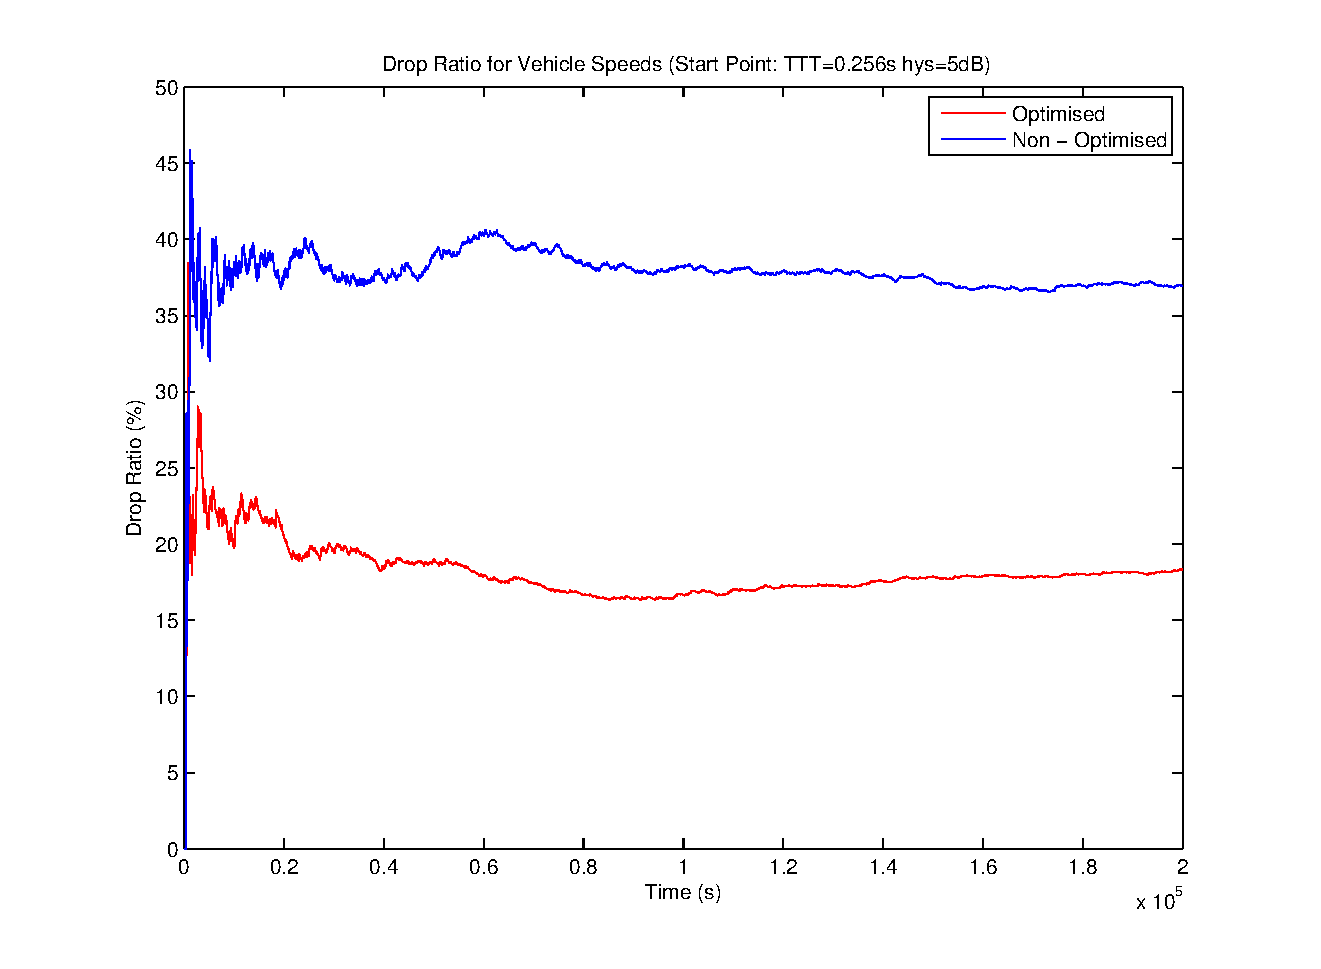
\includegraphics[width=0.75\textwidth]{figures/vehicle_figures/mid/long_drop.eps}
    \end{center}
    \caption{Graph of Optimised vs. Non-Optimised Results for Starting Point TTT=0.256s hys=5dB when UE traveling at vehicle speeds.}
    \label{fig:veh_mid_drop}
\end{figure}

\begin{figure}[H]
        \centering
        \begin{subfigure}[b]{0.49\textwidth}
                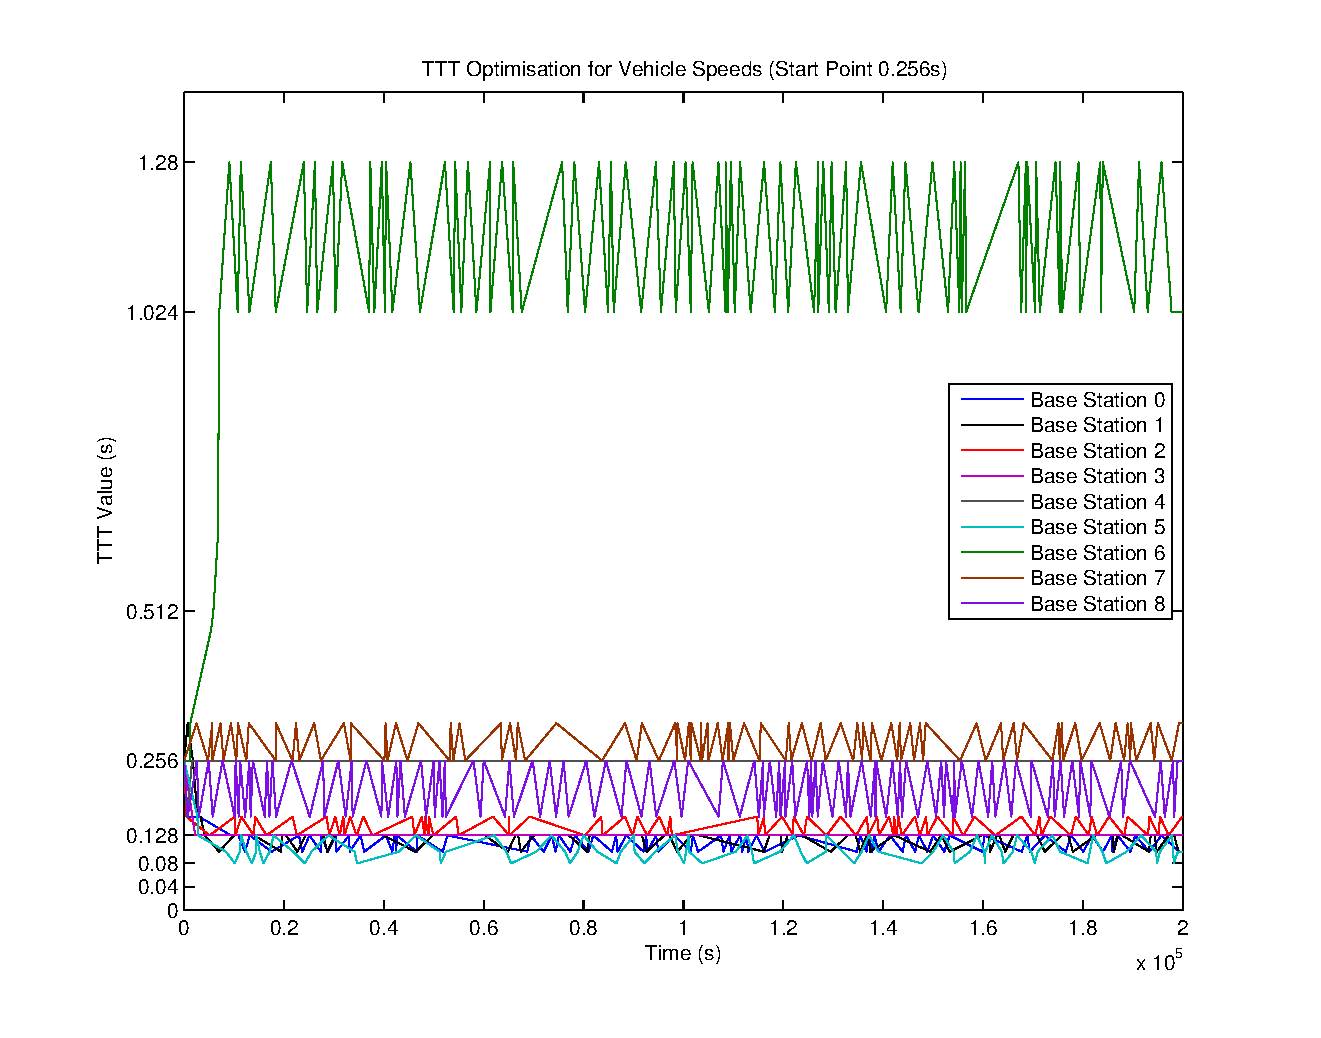
\includegraphics[width=\textwidth]{figures/vehicle_figures/mid/long_ttt.eps}
                \caption{Changing TTT Values}
                \label{fig:veh_mid_ttt}
        \end{subfigure}%
        ~ %add desired spacing between images, e. g. ~, \quad, \qquad etc.
          %(or a blank line to force the subfigure onto a new line)
        \begin{subfigure}[b]{0.49\textwidth}
                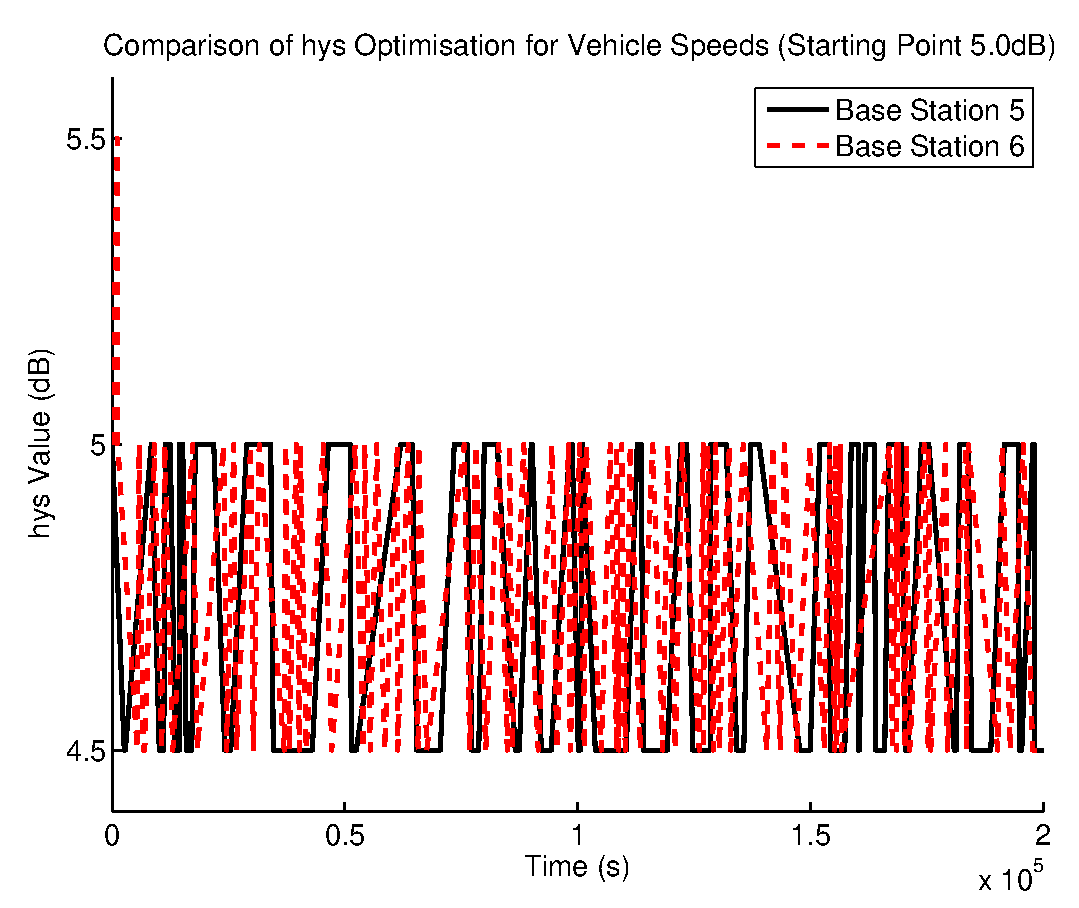
\includegraphics[width=\textwidth]{figures/vehicle_figures/mid/long_hys.eps}
                \caption{Changing hys Values}
                \label{fig:veh_mid_hys}
        \end{subfigure}
        \caption{Illustration of how the TTT and hys values changed over time for medium values when UE traveling at vehicle speeds.}\label{fig:veh_mid_ttthys}
\end{figure}

\subsubsection*{Small Values}
\begin{figure}[H]
  \begin{center}
    	  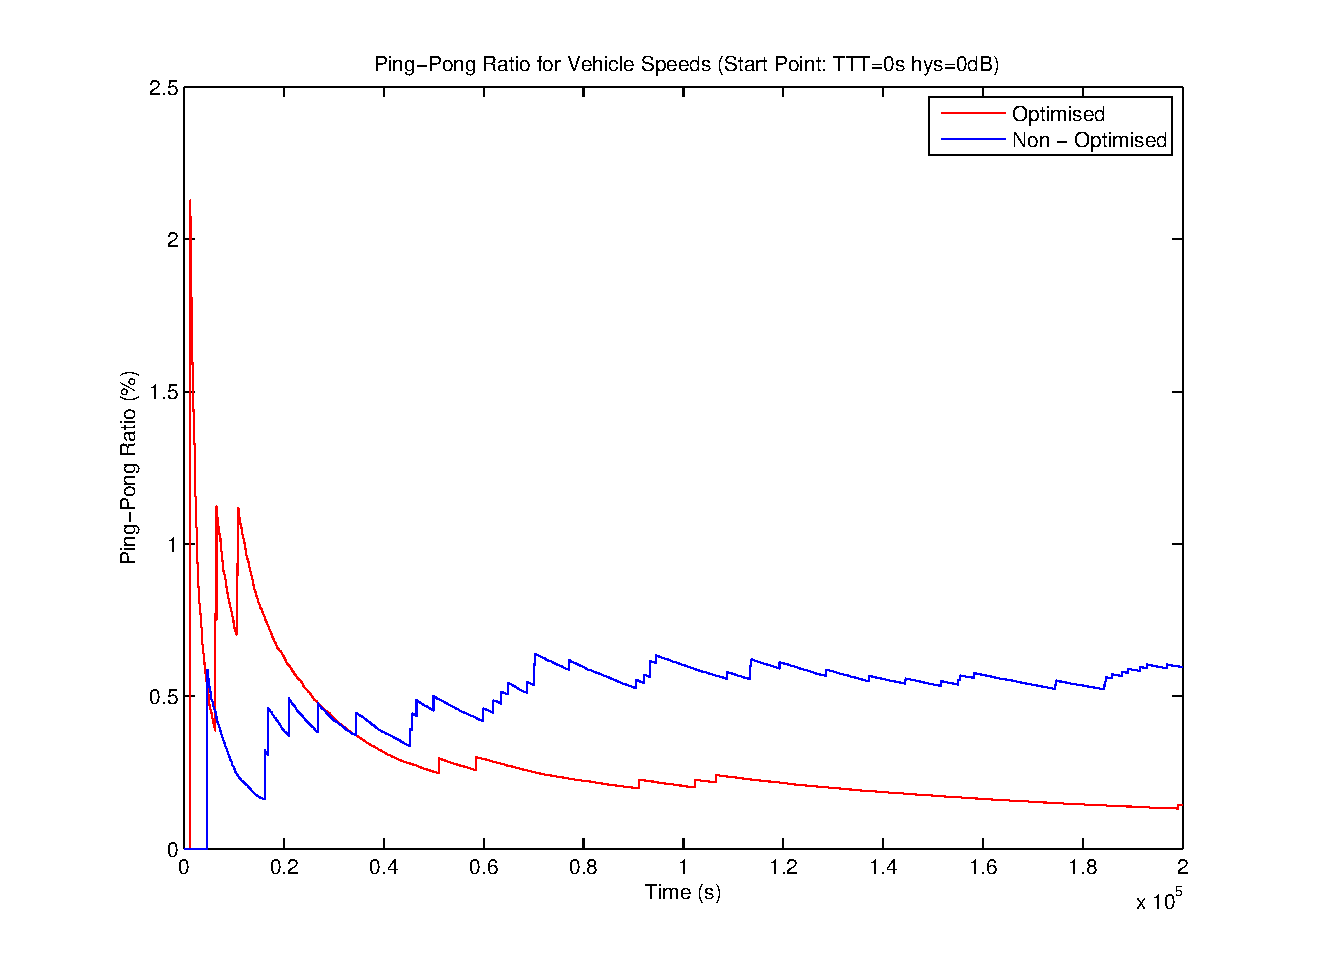
\includegraphics[width=0.75\textwidth]{figures/vehicle_figures/low/long_ping.eps}
    \end{center}
    \caption{Graph of Optimised vs. Non-Optimised Results for Starting Point TTT=0s hys=0dB when UE traveling at vehicle speeds.}
    \label{fig:veh_low_drop}
\end{figure}

\begin{figure}[H]
        \centering
        \begin{subfigure}[b]{0.49\textwidth}
                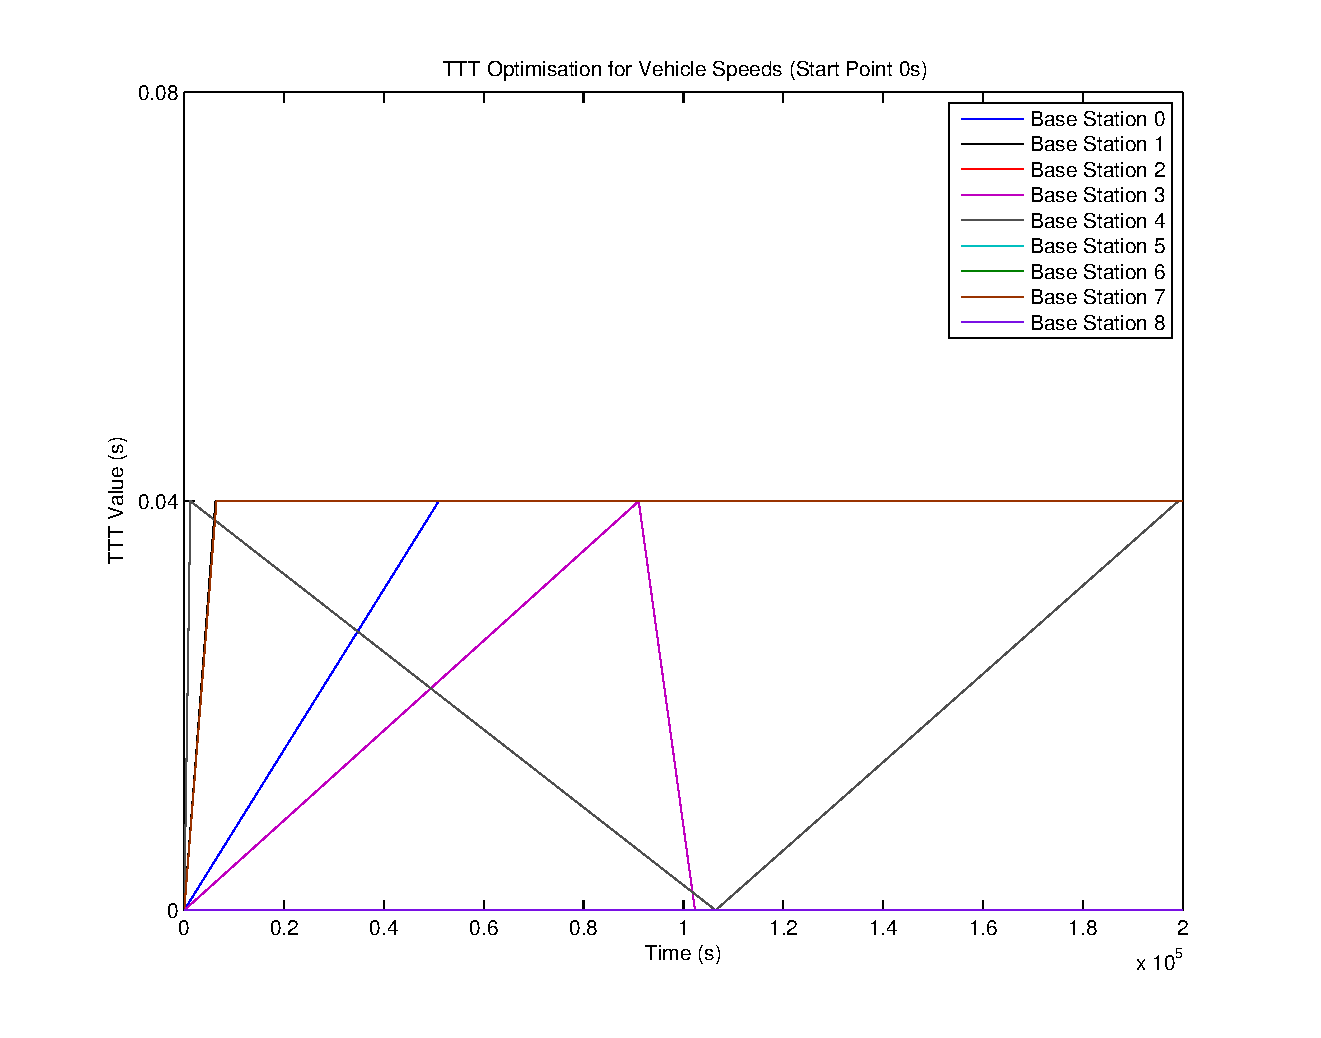
\includegraphics[width=\textwidth]{figures/vehicle_figures/low/long_ttt.eps}
                \caption{Changing TTT Values}
                \label{fig:veh_low_ttt}
        \end{subfigure}%
        ~ %add desired spacing between images, e. g. ~, \quad, \qquad etc.
          %(or a blank line to force the subfigure onto a new line)
        \begin{subfigure}[b]{0.49\textwidth}
                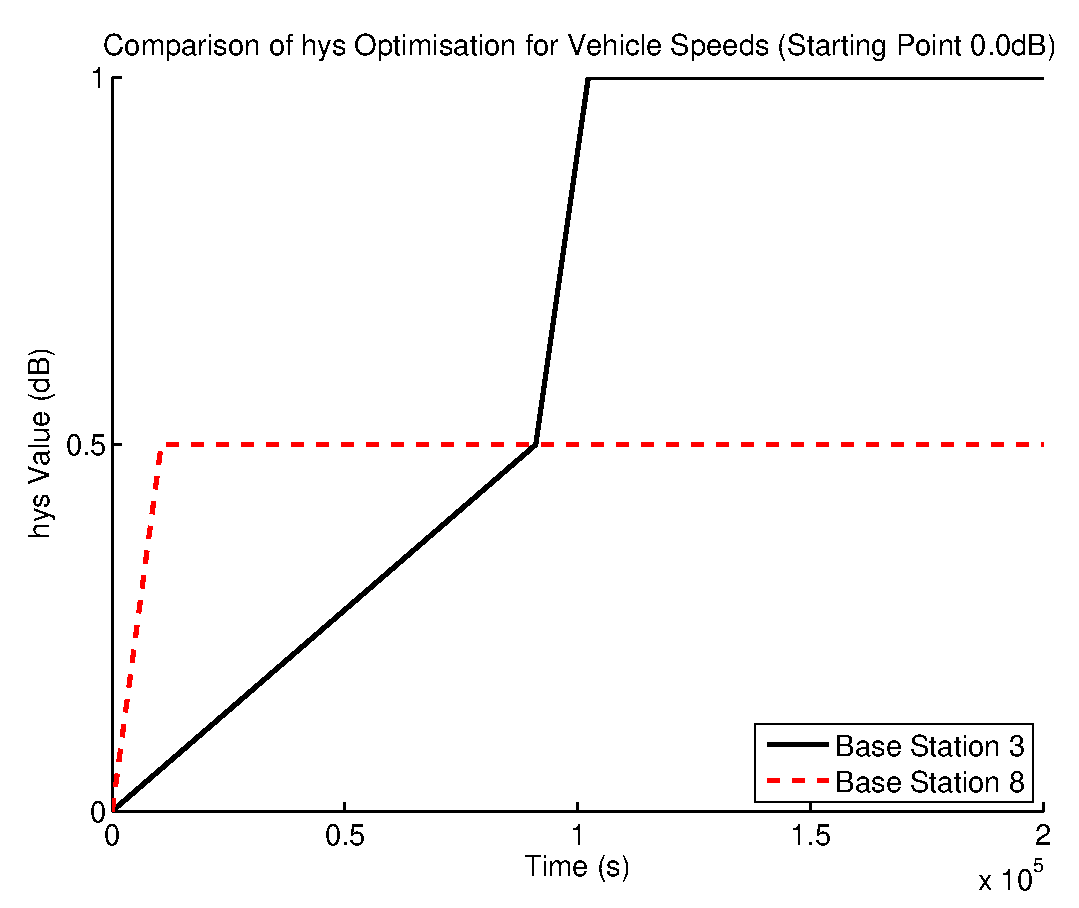
\includegraphics[width=\textwidth]{figures/vehicle_figures/low/long_hys.eps}
                \caption{Changing hys Values}
                \label{fig:veh_low_hys}
        \end{subfigure}
        \caption{Illustration of how the TTT and hys values changed over time for medium values when UE traveling at vehicle speeds.}\label{fig:vel_low_ttthys}
\end{figure}

\subsubsection*{Large hys and Small TTT Values}
\begin{figure}[H]
  \begin{center}
    	  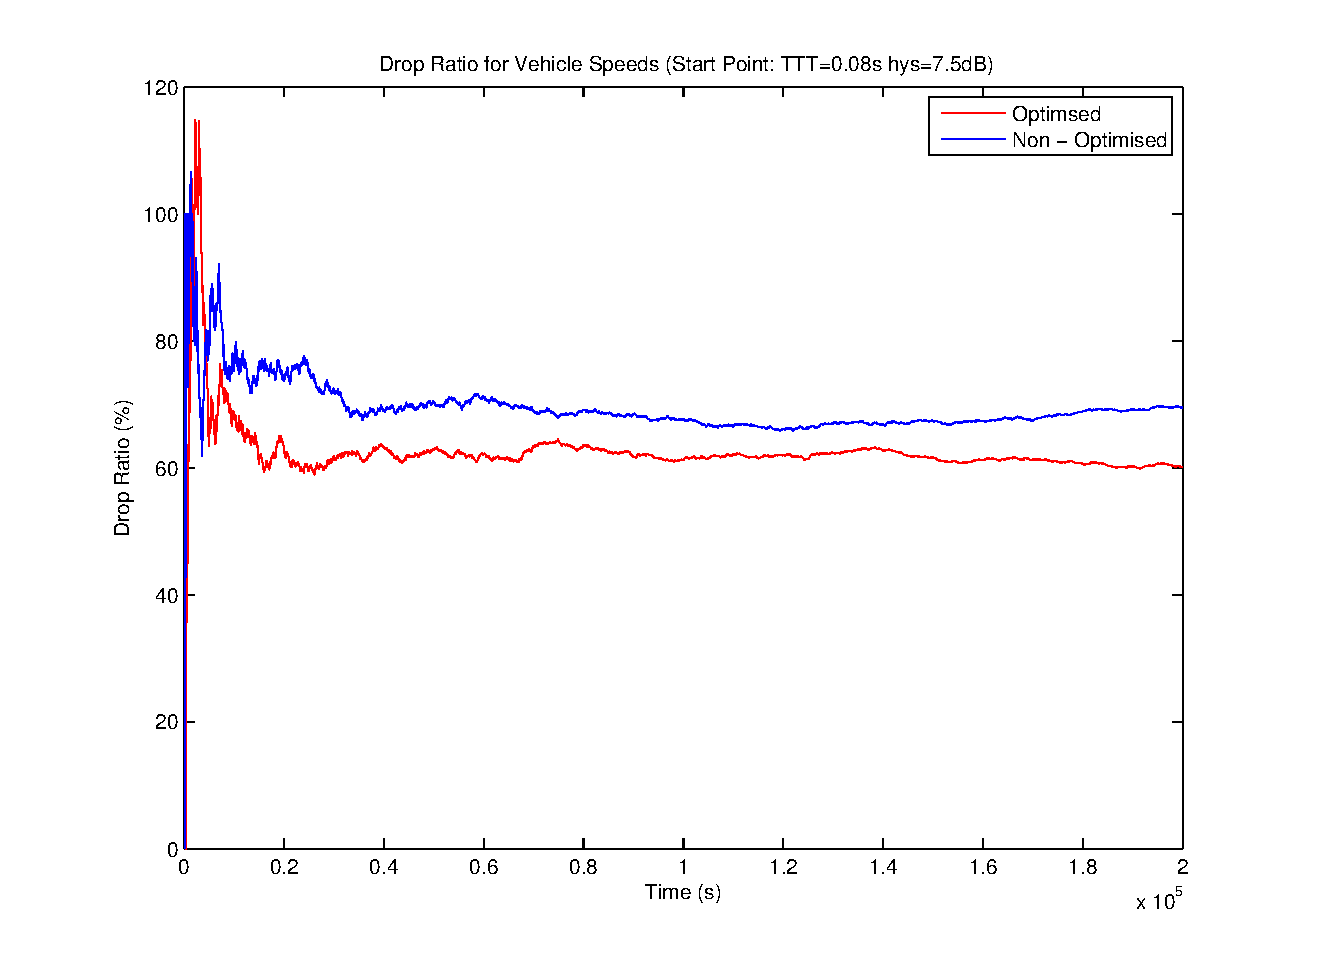
\includegraphics[width=0.75\textwidth]{figures/vehicle_figures/highhys/long_drop.eps}
    \end{center}
    \caption{Graph of Optimised vs. Non-Optimised Results for Starting Point TTT=0.08s hys=7.5dB when UE traveling at vehicle speeds.}
    \label{fig:veh_highhys_drop}
\end{figure}

\begin{figure}[H]
        \centering
        \begin{subfigure}[b]{0.49\textwidth}
                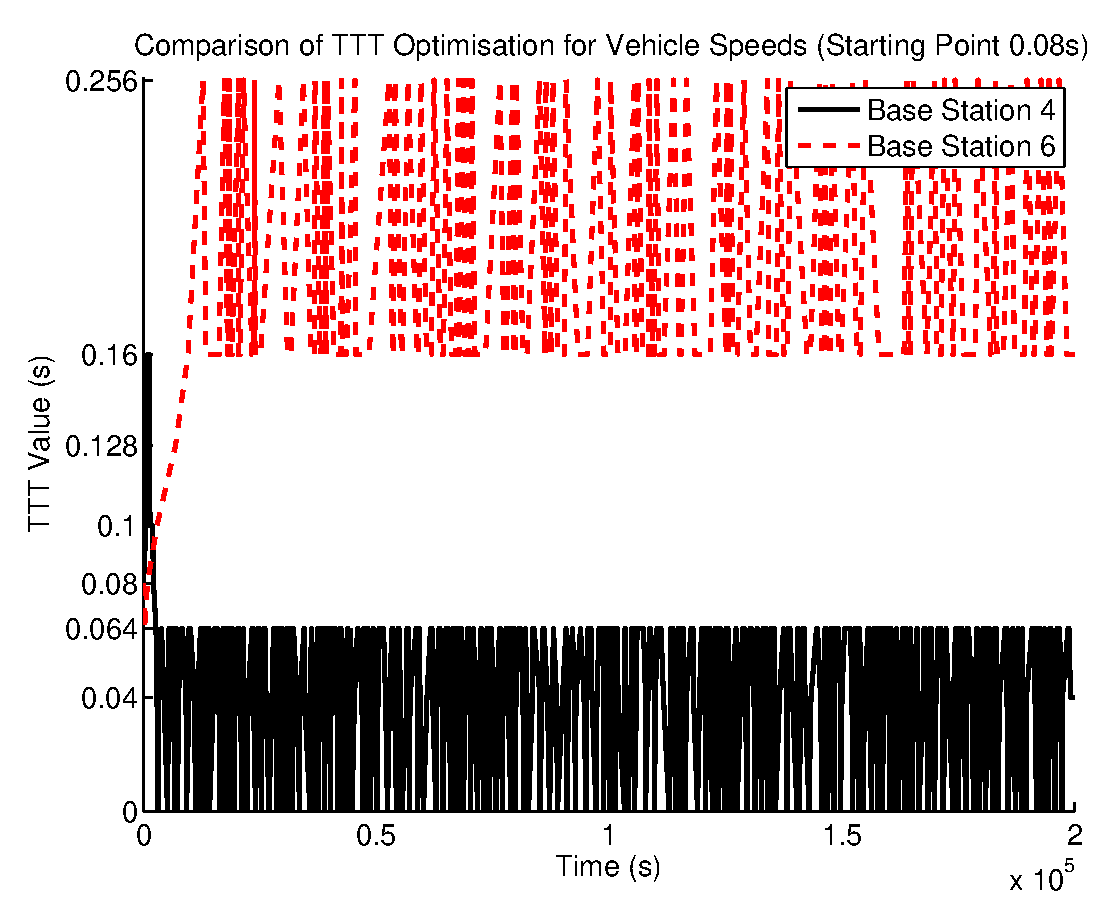
\includegraphics[width=\textwidth]{figures/vehicle_figures/highhys/long_ttt.eps}
                \caption{Changing TTT Values}
                \label{fig:veh_highhys_ttt}
        \end{subfigure}%
        ~ %add desired spacing between images, e. g. ~, \quad, \qquad etc.
          %(or a blank line to force the subfigure onto a new line)
        \begin{subfigure}[b]{0.49\textwidth}
                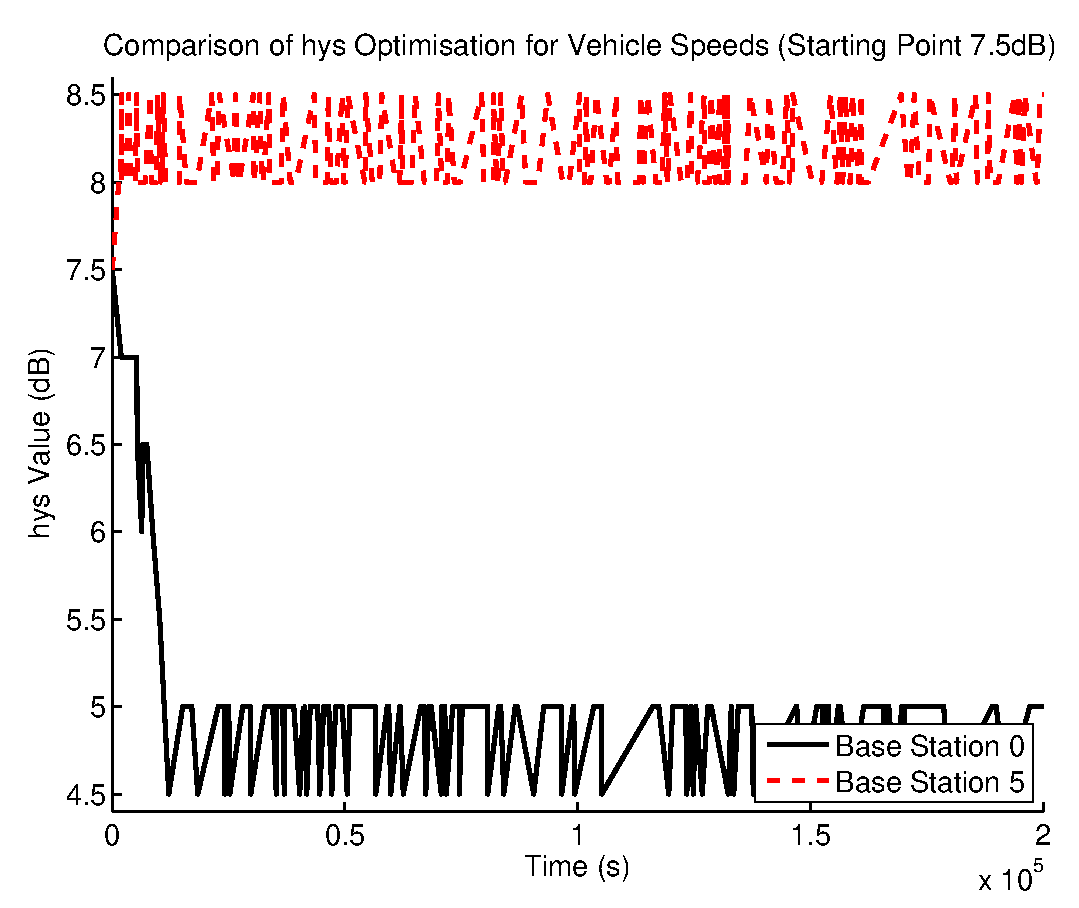
\includegraphics[width=\textwidth]{figures/vehicle_figures/highhys/long_hys.eps}
                \caption{Changing hys Values}
                \label{fig:veh_highhys_hys}
        \end{subfigure}
        \caption{Illustration of how the TTT and hys values changed over time for medium values when UE traveling at vehicle speeds.}\label{fig:veh_highhys_ttthys}
\end{figure}